%Descrever o cronograma previsto para a realização dos passos definidos na Metodologia com resolução em nível de semanas.
%Roadmap
%
%- Implementação
%  - Parser 		OK
%  - Estrutura 		OK
%  - Utilidades 		WIP
%	09/04 -> 15/04
%  - Metodos Antigos	0%
%	16/04 -> 23/04
%  - Metodos Novos	0%
%	23/04 -> 29/04
%  - Operadores		0%
%	30/04 -> 06/04
%- Comparacao dos metodos
%  - Modelagem e analise usando metodo tradicional
%	07/05 -> 13/05
%  - Modelagem e analise usando metodo aproximativo
%	14/05 -> 20/05
%- Restantes
%  - Escrever o relatorio
%  - Poster
%  - Apresentacao parcial e final
%  - Bugfixes e melhorias

O cronograma(Fig. 1) foi definido dividindo as etapas em blocos de semana, e pelo planejado a implementação e a análise deve estar pronta na época da apresentação parcial.

\begin{figure}[h]
\centering
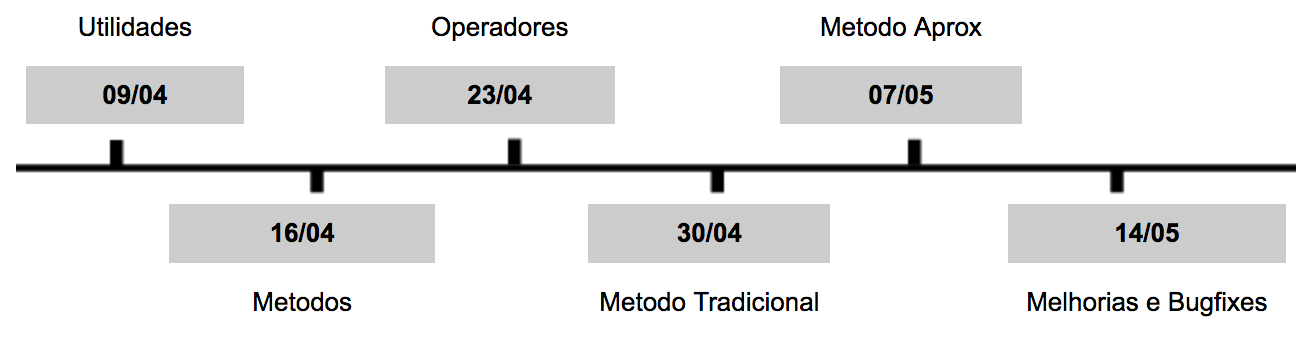
\includegraphics[width=\textwidth]{roadmap.png}
\caption{Cronograma}
\end{figure}

Do dia 14/05 para frente será reservado para melhorar a usabilidade da biblioteca e resolver eventuais problemas.
